% ju 31-Dez-22
\documentclass[a4paper,12pt,fleqn,parskip=half]{scrartcl}
\usepackage[ngerman]{babel}
\usepackage[utf8]{inputenc}
\usepackage[T1]{fontenc}

% Schrift
%\usepackage{lmodern}
\usepackage[osf,sc]{mathpazo} 
\usepackage[scale=.9,semibold]{sourcecodepro}   
\usepackage[osf]{sourcesanspro}  

\usepackage[headsepline]{scrlayer-scrpage}
\pagestyle{scrheadings}
\clearpairofpagestyles

\usepackage[table,dvipsnames,usenames]{xcolor}
\usepackage{textcase}
\usepackage{nameref}
\usepackage{hyperref}
\usepackage{tabularx}
\usepackage{multirow}
\usepackage{multicol}
\usepackage{caption, booktabs}
\usepackage{graphicx} 
\usepackage{scrhack}    
\usepackage{url}%% Links
\usepackage[inline]{enumitem}
\usepackage{pifont}
\usepackage{eurosym}% \euro 20,-
\usepackage{amsmath}
\usepackage{amsfonts}
\usepackage{amssymb}
\usepackage{array}            % Extending the array and tabular environments
\usepackage{chngcntr}         % Change the resetting of counters
\usepackage[version=4]{mhchem}
\usepackage{stmaryrd}
\usepackage{siunitx}
\usepackage{float}
\usepackage{csquotes}
\usepackage{subcaption}
\usepackage{mathtools}
\usepackage{icomma}%Dezimaltrennzeichen
\usepackage{multimedia}%Video: \movie[externalviewer]{(video.mov)}{video.mov}
\usepackage{epstopdf}
\usepackage{footnote}
\usepackage{qrcode}% Anwendung: \qrcode[hyperlink,level=Q,version=2,height=1cm]{\website}
\usepackage{underscore}% Unterstrich ____

% PDF Dokumente einbinden
\usepackage{pdfpages}% \includepdf[pages=-]{Tabellen/Excel.pdf}
\RequirePackage{lastpage}  % Pagecounter

\addto\captionsngerman{%
\renewcommand{\figurename}{Abb.}
\renewcommand{\tablename}{Tab.}
}

% listings
\usepackage{listings}
\lstset{basicstyle=\linespread{1}\ttfamily\small,floatplacement=!htb,captionpos=t,abovecaptionskip=.5\baselineskip,belowcaptionskip=.5\baselineskip,upquote=true,showstringspaces=false,inputencoding=utf8,tabsize=4,
    	keywordstyle=\bfseries ,
	commentstyle=\color{rot5},
	stringstyle=\color{orange},
	breaklines=true,
  	postbreak=\mbox{\textcolor{black}{$\hookrightarrow$}\space},
	breakatwhitespace=false
}
\lstset{literate={á}{{\'a}}1 {é}{{\'e}}1 {í}{{\'i}}1 {ó}{{\'o}}1 {ú}{{\'u}}1 {Á}{{\'A}}1 {É}{{\'E}}1 {Í}{{\'I}}1 {Ó}{{\'O}}1 {Ú}{{\'U}}1 {à}{{\`a}}1 {è}{{\`e}}1 {ì}{{\`i}}1 {ò}{{\`o}}1 {ù}{{\`u}}1 {À}{{\`A}}1 {È}{{\'E}}1 {Ì}{{\`I}}1 {Ò}{{\`O}}1 {Ù}{{\`U}}1 {ä}{{\"a}}1 {ë}{{\"e}}1 {ï}{{\"i}}1 {ö}{{\"o}}1 {ü}{{\"u}}1 {Ä}{{\"A}}1 {Ë}{{\"E}}1 {Ï}{{\"I}}1 {Ö}{{\"O}}1 {Ü}{{\"U}}1 {â}{{\^a}}1 {ê}{{\^e}}1 {î}{{\^i}}1 {ô}{{\^o}}1 {û}{{\^u}}1 {Â}{{\^A}}1 {Ê}{{\^E}}1 {Î}{{\^I}}1 {Ô}{{\^O}}1 {Û}{{\^U}}1 {œ}{{\oe}}1 {Œ}{{\OE}}1 {æ}{{\ae}}1 {Æ}{{\AE}}1 {ß}{{\ss}}1 {ű}{{\H{u}}}1 {Ű}{{\H{U}}}1 {ő}{{\H{o}}}1 {Ő}{{\H{O}}}1 {ç}{{\c c}}1 {Ç}{{\c C}}1 {ø}{{\o}}1 {å}{{\r a}}1 {Å}{{\r A}}1 {€}{{\EUR}}1 {£}{{\pounds}}1 {~}{{\textasciitilde}}1 {-}{{-}}1 }

% bibliography
\usepackage[
    bibencoding=utf8,
    backend=biber,% bibtex, biber
    backref=false,backrefstyle=three+,url=true,urldate=comp,abbreviate=false,maxnames=20
]{biblatex} %Paket laden
\DeclareBibliographyCategory{cited}
\let\defaultcite\cite\renewcommand*\cite[2][]{\addtocategory{cited}{#2}\defaultcite[#1]{#2}}
\let\defaulttextcite\textcite\renewcommand*\textcite[2][]{\addtocategory{cited}{#2}\defaulttextcite[#1]{#2}}
\setcounter{biburllcpenalty}{7000}
\setcounter{biburlucpenalty}{8000}
\AfterPackage{biblatex}{
	\PreventPackageFromLoading[\errmessage{Sie haben versucht, das Cite-Paket zu laden, das nicht mit biblatex kompatibel ist.}]{cite}
}

\hypersetup{%
	%pdftitle={\titel},
	%pdfsubject={Latex},
	%pdfauthor={\autor},
	%pdfcreator={\autor}, 
	bookmarksnumbered=true,
	breaklinks=true,
	%colorlinks=true,	   
	linkcolor=rot5,		
	filecolor=blau5,		
	urlcolor=blau5,			
	citecolor=ForestGreen
}

\linespread{1.1}
\setlist{itemsep=0pt}
\widowpenalty10000
\clubpenalty10000
\tolerance1000   

\usepackage[left=2cm,right=2cm,top=1cm,bottom=1cm,includeheadfoot]{geometry}
%\usepackage[left=4cm,right=2cm,top=1cm, bottom=1cm,includeheadfoot]{geometry}
%\usepackage[left=6cm,right=1cm,top=1cm, bottom=1cm,includeheadfoot]{geometry}
%\usepackage[landscape=true,left=2cm,right=2cm,top=1cm,bottom=1cm,includeheadfoot]{geometry}%quer

% eigene Farbe definieren
% Adobe Prozessfarben: CMYK: 100,50,0,35 -> 1,0.5,0,0.35
\definecolor{orange}{cmyk}{0,0.55,0.61,0}   % 0,55,61,0
\definecolor{blau5}{cmyk}{1,0.77,0.1,0.01}  % 100,77,10,
\definecolor{rot5}{cmyk}{0.22,1,1,0.19}     % 22,100,100,19
\definecolor{grau2}{cmyk}{0,0,0,0.1}        % 0,0,0,40
\definecolor{blau}{cmyk}{0.93,0.66,0,0.21}% 

% Literatur
\bibliography{content/literatur}
\bibliography{content/literatur-kfz}
\bibliography{content/literatur-sport}

%%%%%%%%%%%%%%%%%%%%%%%%%%%%%%%%%%%%%%%%%%%%%%%%%%%%%%%
\newcommand{\name}{Jan Unger}
\newcommand{\thema}{12-Schwungrad-Kupplung}
\newcommand{\quelle}{\name}
\newcommand{\website}{https://bw-ju.de/}
\newcommand{\github}{https://github.com/ju1-eu}
%%%%%%%%%%%%%%%%%%%%%%%%%%%%%%%%%%%%%%%%%%%%%%%%%%%%%%%

\ihead{\textbf{Quelle:} \quelle}%{Kopfzeile innen}
\ohead{\textbf{Datum:} \today}  %{Kopfzeile außen}
\ifoot{\textbf{Thema:} \thema}  %{Fußzeile  innen}
\ofoot{Seite {\thepage} von {\pageref{LastPage}}}%{Fußzeile  außen}

\title{\thema}
\author{\name}
\date{\today}

\begin{document}
	%%%%%%%%%%%%%%%%%%%%%%%%%%%%%%%%%%%%%%%%%%%%%%%%%%%%%%%%%%%%%%%%%%
	\begin{abstract}
		\center
		\textbf{\Large \thema}%14pt
		
		\vspace{1.5em}
		%\datum	
		%\qrcode[hyperlink,level=Q,version=2,height=1cm]{\website}
		\qrcode[hyperlink,level=Q,version=2,height=1cm]{\github}
		
		\vspace{1.5em} 
		\raggedright
		\textbf{\large Keywords}
		% Checkliste
		\begin{itemize}[label=\checkmark]
			\item Begriff
		\end{itemize}
	\end{abstract}
    %%%%%%%%%%%%%%%%%%%%%%%%%%%%%%%%%%%%%%%%%%%%%%%%%%%%%%%%%%%%%%%%%%

	% anpassen
	%\input{content/tex/neu}
	%ju 31-Dez-22 12-Schwungrad-Kupplung.tex
\section{Antriebsarten}\label{antriebsarten}

\textbf{Nenne Merkmale eines Hinterradantriebs}

Die Antriebsleistung wird von den Rädern der Hinterachse auf die Straße
übertragen.

\begin{enumerate}
\item
  Gelenkwellentunnel im Fahrgastraum
\item
  Günstige Gewichtsverteilung zwischen Vorder- und Hinterachse
\item
  Die Vorderräder übertragen hohe Seitenführungskräfte, da an Ihnen nur
  die Lenkkräfte angreifen
\item
  Erhöhung der Traktion beim Beschleunigen und Bergauffahrten, da die
  Radlast durch die dynamische Achslastverteilung zunimmt
\end{enumerate}

\textbf{Nenne Merkmale eines Vorderradantriebs}

Beim Vorderradantrieb wird die Antriebsleistung von den Vorderrädern
übertragen.

\begin{enumerate}
\item
  Die Übertragung der Seitenführungskräfte an der Vorderachse ist
  verringert, da auch die Antriebskräfte an den Rädern diese Achse
  angreifen
\item
  Beim Beschleunigen vermindern sich die Seitenführungskraft und die
  Traktion an den Antriebsrädern, da dabei die Räder der Vorderachse
  entlastet werden
\item
  Unterschiedlich auftretende Kräfte an den Rädern beeinflussen das
  Lenkverhalten
\end{enumerate}

\section{Kupplung}\label{kupplung}

\textbf{Nenne Aufgaben der Kupplung}

\begin{enumerate}
\item
  Motordrehmoment übertragen
\item
  weiches und ruckfreies Anfahren ermöglichen
\item
  Drehschwingungen zu dämpfen
\item
  Kraftfluss beim Schaltvorgang unterbrechen
\item
  Drehzahldifferenzen nach dem Schalten anpassen
\item
  Anhalten des Fahrzeugs bei laufendem Verbrennungsmotor ermöglichen
\end{enumerate}

\textbf{Welche Arten von Reibungskupplungen gibt es?}

\begin{enumerate}
\item
  Einscheibenkupplung
\item
  Zweischeibenkupplung

  \begin{itemize}
  \item
    Anwendung: Erhöhung des übertragbaren Drehmoments und zur Minderung
    des Verschleißes bei häufiger Kupplungsbetätigung
  \end{itemize}
\item
  Lamellenkupplung
\item
  Fliehkraftkupplung
\end{enumerate}

\textbf{Welche Arten von Strömungskupplungen gibt es?}

\begin{enumerate}
\item
  Hydrodynamische Kupplung
\item
  Hydrodynamischer Drehmomentwandler
\end{enumerate}

\textbf{Wovon ist das übertragbare Drehmoment einer Kupplung abhängig?}

\begin{enumerate}
\item
  Anpresskraft der Federn
\item
  Reibungszahl / Reibwert der Reibpaarungen (Schwungrad -- Reibbelag --
  Druckplatte),
\item
  mittlere Radius (dem wirksamen Hebelarm) $M_k = F_R \cdot r_m$
\item
  Anzahl der Reibbeläge / Reibflächen (Einscheibenkupplung: 2)
\end{enumerate}

\section{Mechanische Kupplungsbestätigung ohne
Selbstnachstellung}\label{mechanische-kupplungsbestaetigung-ohne-selbstnachstellung}

\begin{figure}[!ht]% hier: !ht
\centering
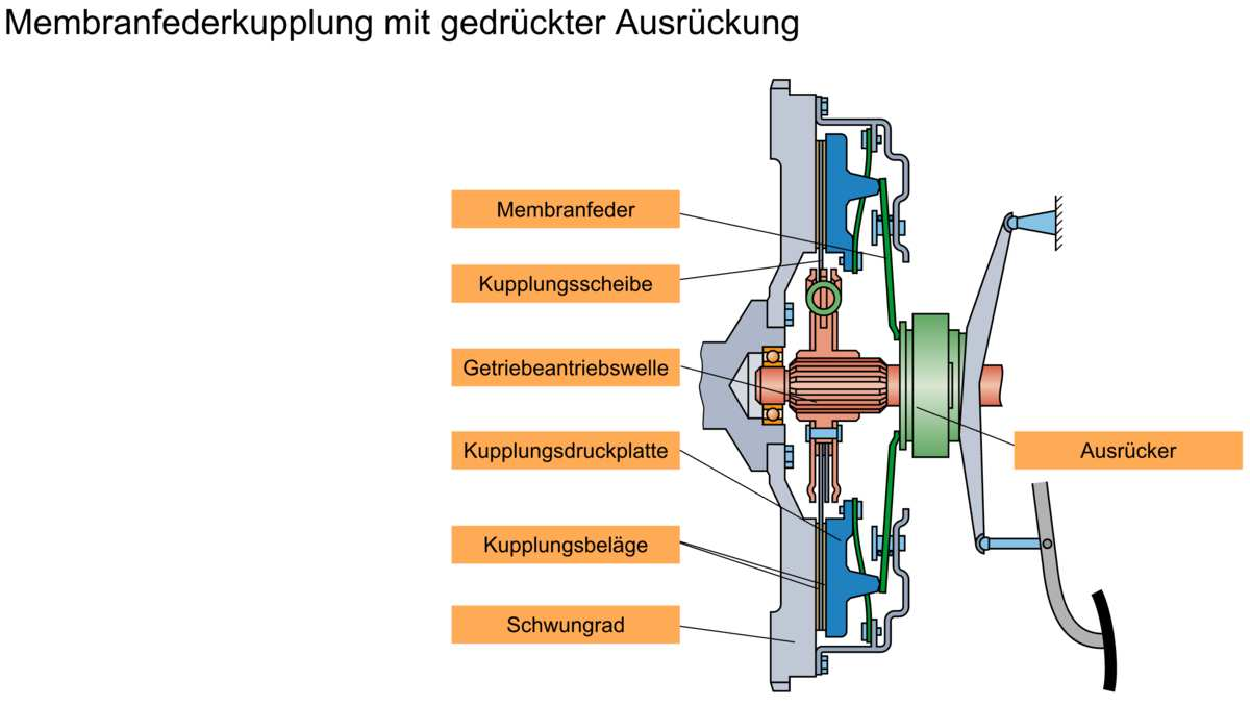
\includegraphics[width=0.7\textwidth]{images/Kupplung/Kupplung-8.pdf}
\caption{Kupplung, Quelle: Europa-Verlag}
%\label{fig:}%% anpassen
\end{figure}

Faktor 10, Ausrückhebel und Membranfederzungen 1 -- 3 mm, Leerweg am
Pedal 10 -- 30 mm

\textbf{manuellen Nachstellung}, das Seil wird mithilfe eines Gewindes
in eine neue Position gebracht. Am Pedal sollte ein Leerweg von etwa 10
bis 30 mm bleiben, um wärmebedingte Ausdehnungen zu kompensieren.

\textbf{Auswirkung von zu kleinem Kupplungsspiel}

\begin{enumerate}
\item
  Rutschen der Kupplung wegen geringer Anpresskraft der Membranfeder
\item
  Überhitzung der Kupplungsbeläge
\item
  Ausglühen der Membranfeder
\item
  Einlaufen der Membranfederspitzen
\item
  Punktuelle Überhitzung der Reibfläche am Schwungrad
\end{enumerate}

\textbf{Kraftfluss im eingekuppelten Zustand}

Kurbelwelle $\to$ Schwungrad $\to$ Druckplatte $\to$
Kupplungsscheibe $\to$ Getriebeantriebswelle

\textbf{Beschreibe den Vorgang des Auskuppelns}

\begin{enumerate}
\item
  Das Ausrücklager wird gegen den Innenrand der Membranfederzungen
  gedrückt.
\item
  Die Membranfeder wird in den Kippringen gekippt.
\item
  Die vorgespannten Tangentialplattfedern heben die Druckplatte ab.
\item
  Der Kraftfluss ist unterbrochen.
\end{enumerate}

\newpage

\section{Hydraulische
Kupplungsbetätigung}\label{hydraulische-kupplungsbetaetigung}

\begin{figure}[!ht]% hier: !ht
\centering
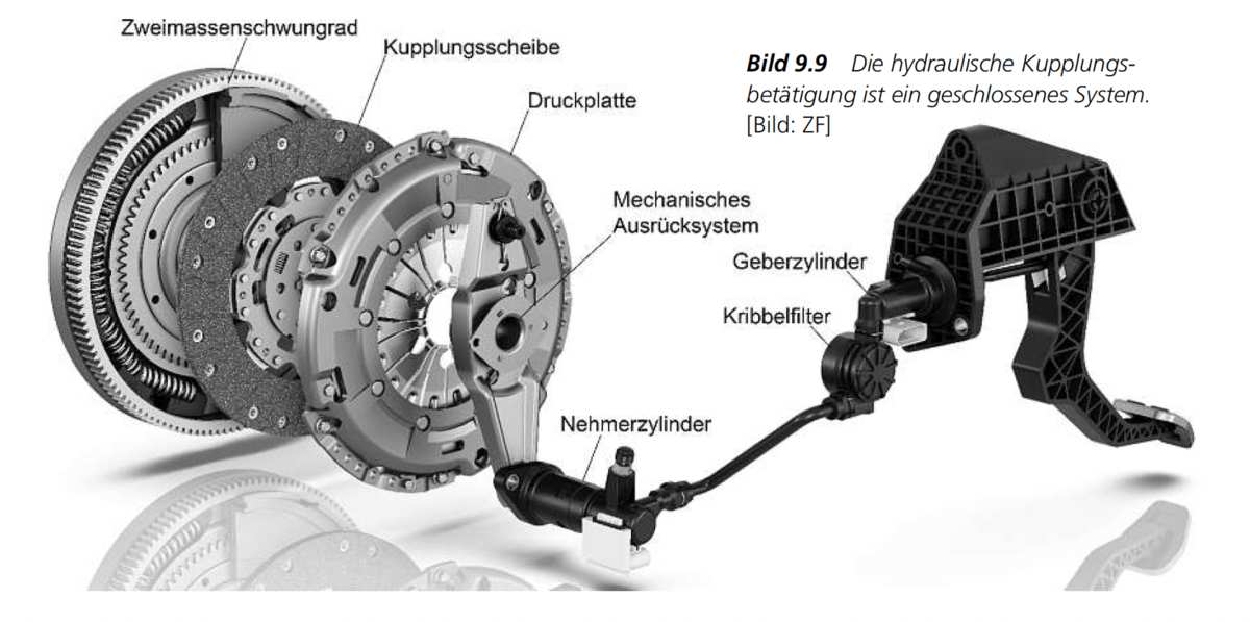
\includegraphics[width=0.7\textwidth]{images/Kupplung/Kupplung-1.pdf}
\caption{Hydraulische Kupplungsbetätigung, Quelle: Respondek}
%\label{fig:}%% anpassen
\end{figure}

\textbf{Vorteile}

\begin{enumerate}
\item
  Verstärkung durch hydraulische Übersetzung
\item
  Einfache Verlegung
\end{enumerate}

Der \textbf{Geberzylinder} erzeugt den Druck, der über den
\textbf{Nehmerzylinder} auf den Ausrückhebel, oder zentral geführt
direkt auf das Ausrücklager wirkt. In Ruhelage ist der Geberzylinder
über die Ausgleichsbohrung mit dem Ausgleichsbehälter, oftmals der von
der Bremse, verbunden. Somit kann die mit zunehmendem Belagverschleiß
überflüssige Bremsflüssigkeit dorthin entweichen und das System wird
selbstnachstellend. Bei einigen wenigen Fahrzeugen ist dennoch eine
Nachstellung des Endanschlags am Nehmerzylinder erforderlich.

Das System besitzt einen sog. Kribbelfilter (Schwingungsdämpfer), da der
Verbrennungsmotor die Kupplung durch seine Arbeitstakte zu Schwingungen
anregen kann, die sich durch das Ausrücksystem bis in das Pedal
fortsetzen. Diese Schwingungen würde der Fahrer als Kribbeln im Fuß
wahrnehmen.

\newpage

\section{Selbsteinstellende Kupplung (SAC -- Self Adjusting
Clutch)}\label{selbsteinstellende-kupplung-sac-self-adjusting-clutch}

\begin{figure}[!ht]% hier: !ht
\centering
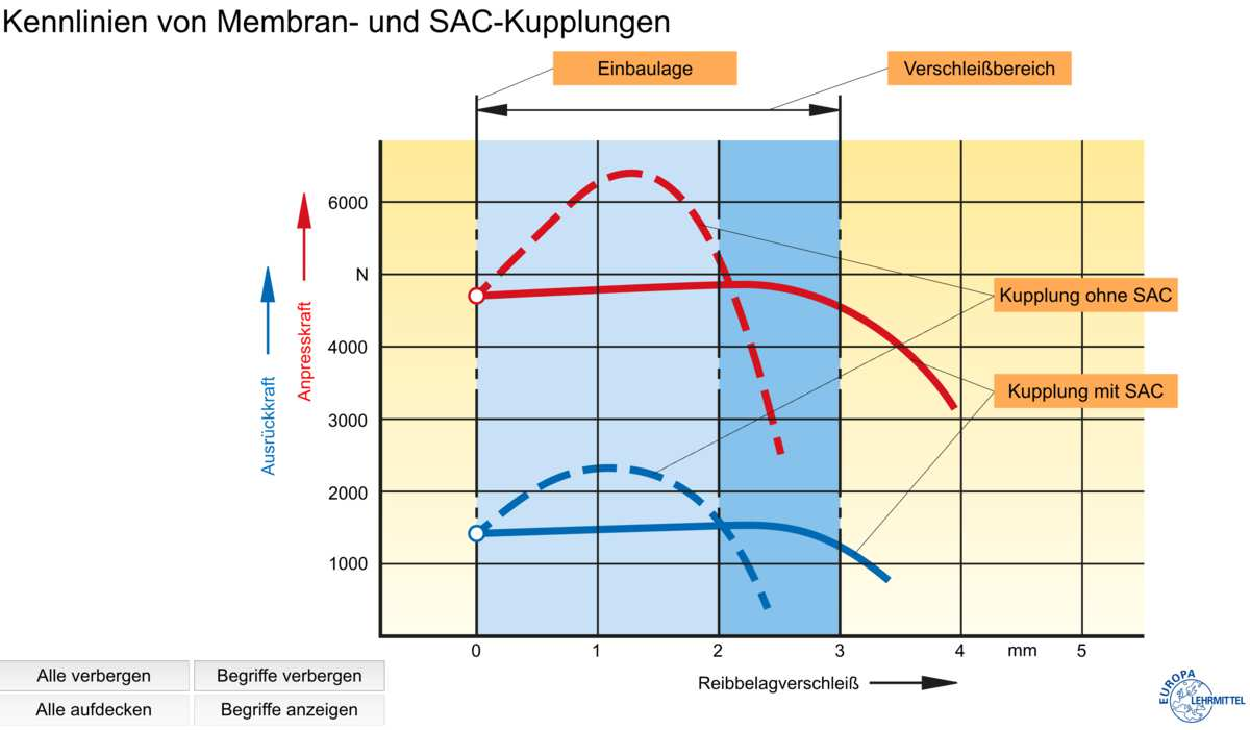
\includegraphics[width=0.7\textwidth]{images/Kupplung/Kupplung-6.pdf}
\caption{Kennlinien von Membran- und SAC-Kupplungen, Quelle:
Europa-Verlag}
%\label{fig:}%% anpassen
\end{figure}

\textbf{Vorteil}

\begin{itemize}
\item
  Schleifpunkt der Kupplung und die erforderliche Ausrückkraft, Pedal-
  und Anpresskräfte bleiben über den Belagverschleiß nahezu gleich.
  Größerer Belagverschleiß möglich.
\item
  die Kupplung stellt sich bei Belagverschleiß selbsttätig nach
\end{itemize}

\begin{figure}[!ht]% hier: !ht
\centering
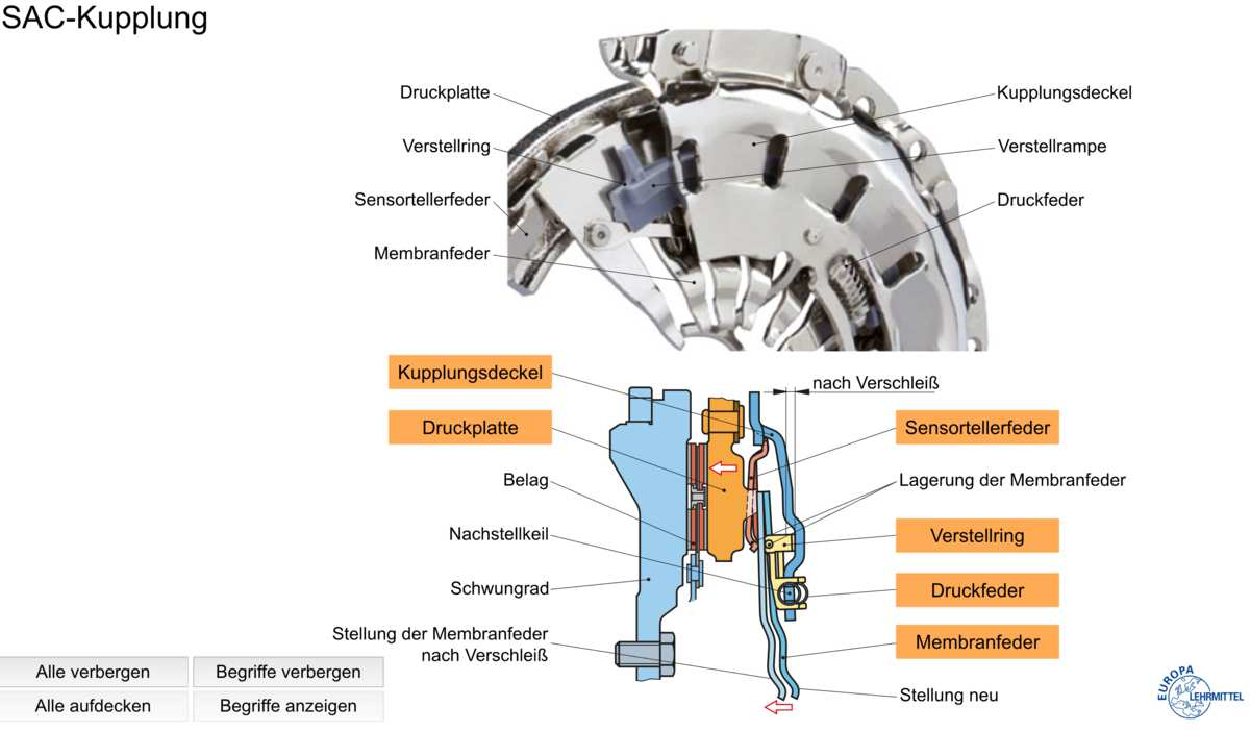
\includegraphics[width=0.7\textwidth]{images/Kupplung/Kupplung-7.pdf}
\caption{Selbsteinstellende Kupplung (SAC), Quelle: Europa-Verlag}
%\label{fig:}%% anpassen
\end{figure}

Durch eine Kombination der Membranfeder mit einer Sensor-Tellerfeder und
einem Verstellring.

\section{Kupplungsscheiben}\label{kupplungsscheiben}

\textbf{Nenne Aufgaben von Kupplungsscheiben}

\begin{enumerate}
\item
  Motordrehmomente übertragen vom Schwungrad auf die
  Getriebeeingangswelle
\item
  weiches und ruckfreies Anfahren ermöglichen
\item
  Drehschwingungen dämpfen
\end{enumerate}

\textbf{Welche Aufgabe haben die Belagfedern einer Kupplungsscheibe?}

\begin{itemize}
\item
  weiches und ruckfreies Anfahren ermöglichen
\item
  gleicht minimale Unebenheiten des Schwungrades und der Druckplatte
  aus, die ein Durchrutschen der Kupplung auslösen würde
\end{itemize}

\textbf{Welche Aufgabe haben die Torsionsfedern in einer
Kupplungsscheibe?}

\begin{itemize}
\item
  gleicht die Drehschwingungen des Motors aus
\item
  mindert Getriebegeräusche und Vibrationen
\end{itemize}

\newpage

\section{Störungssuche Kupplung}\label{stoerungssuche-kupplung}

\begin{figure}[!ht]% hier: !ht
\centering
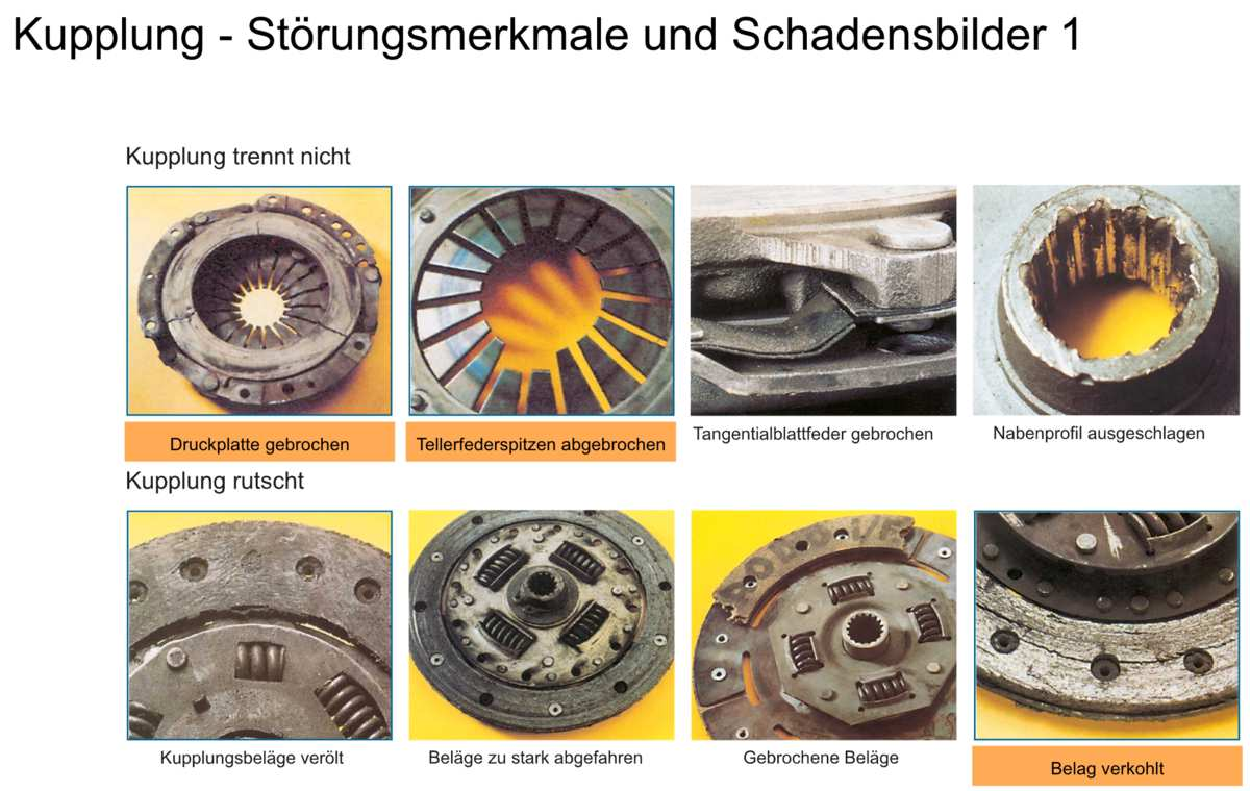
\includegraphics[width=0.7\textwidth]{images/Kupplung/Kupplung-5.pdf}
\caption{Kupplung rutscht oder trennt nicht, Quelle: Europa-Verlag}
%\label{fig:}%% anpassen
\end{figure}

\textbf{Kupplung rutscht}

\begin{enumerate}
\item
  Belag verschlissen
\item
  Belag verölt, verfettet
\item
  Belag überhitzt
\item
  Belag gebrochen
\item
  Schwungrad riefig/überhitzt
\item
  Druckplatte riefig/überhitzt
\item
  Kupplungsbetätigung schwergängig oder falsch eingestellt
\item
  Feder(n) gebrochen
\item
  SAC falsch eingebaut/eingestellt
\end{enumerate}

\textbf{Kupplung trennt nicht}

\begin{enumerate}
\item
  ZMS hat erhöhtes Axialspiel
\item
  Kupplungsbetätigung falsch eingestellt oder defekt
\item
  Nabe hängt auf der Getriebeeingangswelle (Schmutz/Rost/Beschädigung)
\item
  Seitenschlag der Kupplungsscheibe
\item
  Membranfeder/Ausrückhebel eingelaufen, verzogen oder gebrochen
\item
  Pilotlager schwergängig
\item
  Übermäßiges Axialspiel der Kurbelwelle
\item
  Kupplungsscheibe falsch eingebaut (Getriebe-/Motorseite)
\item
  Falsche Kupplungsscheibe eingebaut
\item
  SAC falsch eingebaut/eingestellt
\end{enumerate}

\textbf{Geräusche aus dem Kupplungsgehäuse}

\begin{figure}[!ht]% hier: !ht
\centering
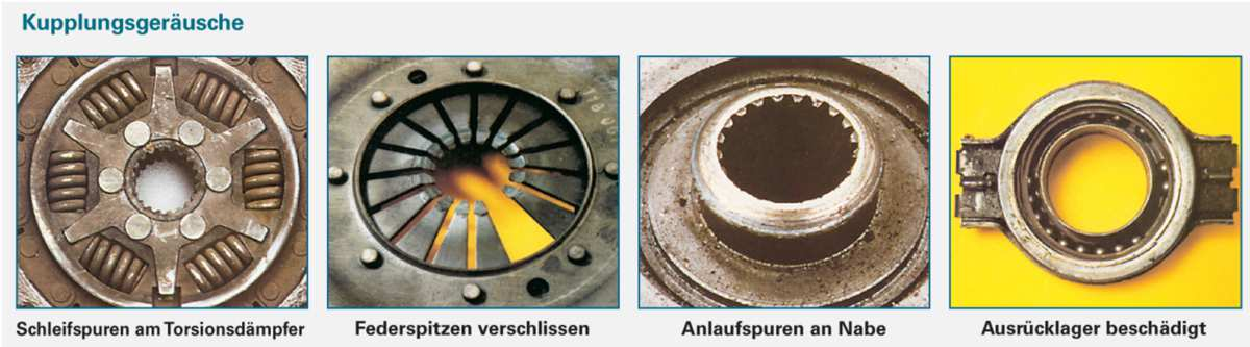
\includegraphics[width=0.7\textwidth]{images/Kupplung/Kupplung-3.pdf}
\caption{Kupplungsgeräusche, Quelle: Europa-Verlag}
%\label{fig:}%% anpassen
\end{figure}

\begin{enumerate}
\item
  ZMS defekt
\item
  Torsionsfeder/-dämpfereinrichtung der Kupplungsscheibe defekt
\item
  Ausrücklager defekt
\item
  Pilotlager defekt (Geräusche nur bei getrennter Kupplung)
\end{enumerate}

\textbf{Kupplung rupft}

\begin{figure}[!ht]% hier: !ht
\centering
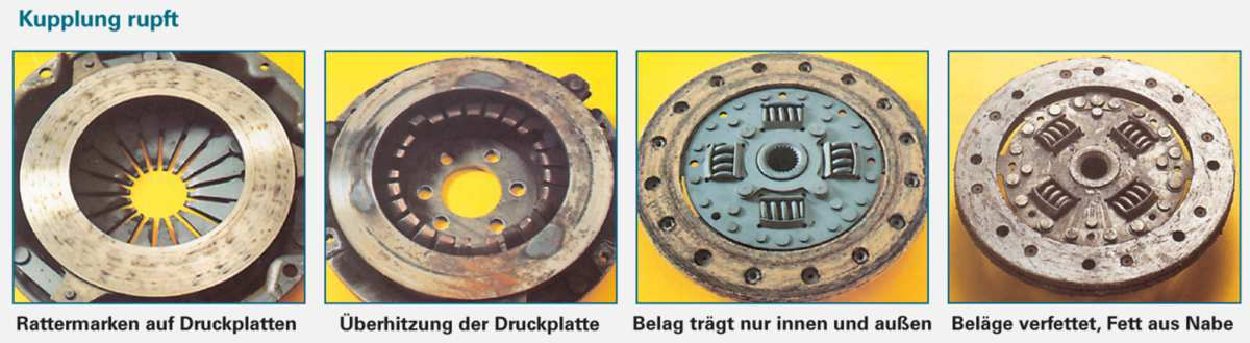
\includegraphics[width=0.7\textwidth]{images/Kupplung/Kupplung-2.pdf}
\caption{Kupplung rupft, Quelle: Europa-Verlag}
%\label{fig:}%% anpassen
\end{figure}

\begin{enumerate}
\item
  Beläge verölt/verfettet
\item
  Schwungrad riefig
\item
  Druckplatte riefig
\item
  Kupplungsgehäuse verzogen
\item
  Erhöhte Torsion im Antriebsstrang (Silentblöcke/Hardyscheibe)
\end{enumerate}

\section{Kupplung prüfen}\label{kupplung-pruefen}

\textbf{Auf Durchrutschen beim Anfahren}

\begin{enumerate}
\item
  Voraussetzung: Motor muss betriebswarm sein
\item
  Fahrzeug durch Feststellbremse sichern
\item
  Auskuppeln und höchsten Vorwärtsgang einlegen
\item
  Motordrehzahl bis zum Drehmomentmaximum erhöhen
\item
  Kupplung schnell einkuppeln und gleichzeitig Gas geben
\end{enumerate}

\textbf{Trennverhalten}

\begin{enumerate}
\item
  Voraussetzung: Motor, Getriebe, Kupplung sollte betriebswarm sein
\item
  Kupplungspedal durchtreten
\item
  3 -- 4 Sekunden warten
\item
  Rückwärtsgang einlegen und auf Geräusche achten
\end{enumerate}

\newpage

\section{Zweimassenschwungrad (ZMS)}\label{zweimassenschwungrad-zms}

\begin{figure}[!ht]% hier: !ht
\centering
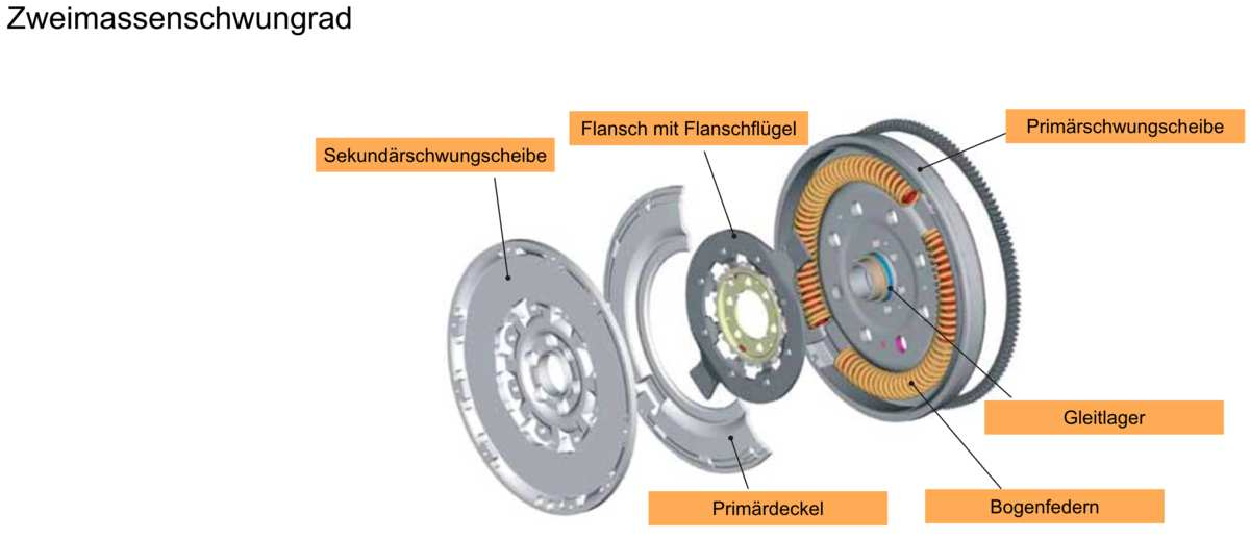
\includegraphics[width=0.7\textwidth]{images/Kupplung/Kupplung-9.pdf}
\caption{Zweimassenschwungrad, Quelle: Europa-Verlag}
%\label{fig:}%% anpassen
\end{figure}

\begin{figure}[!ht]% hier: !ht
\centering
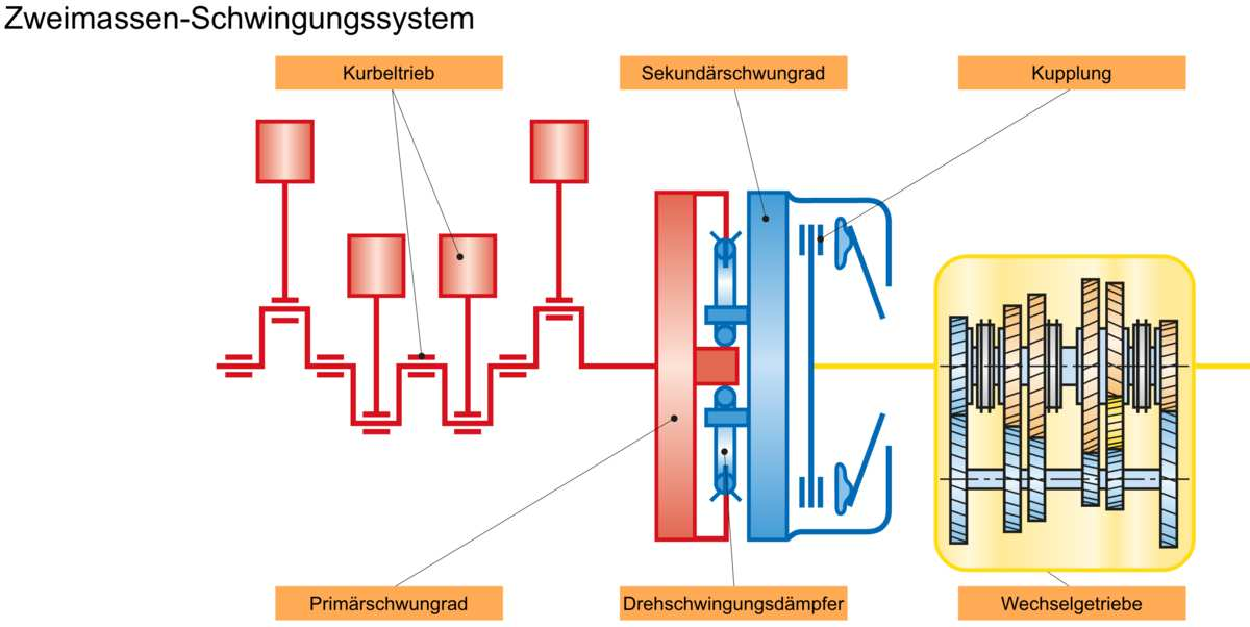
\includegraphics[width=0.7\textwidth]{images/Kupplung/Kupplung-10.pdf}
\caption{Zweimassenschwungrad, Quelle: Europa-Verlag}
%\label{fig:}%% anpassen
\end{figure}

\textbf{Wodurch erfolgt die Dämpfung der Drehschwingungen?}

Durch die Aufteilung der Schwungscheibe in einer Primär- und
Sekundärschwungmasse, die über Bogenfedern verbunden sind.


	%%%%%%%%%%%%%%%%%%%%%%%%%%%%%%%%%%%%%%%%%%%%%%%%%%%%%%%%%%%%%%%%%%
    % Bibliographie
    \printbibliography[category=cited]
\end{document}
